\documentclass[../../main.tex]{subfiles}

\begin{document}

\subsection{Motivation}
Higher order singular value decomposition (HOSVD) can be used as a tool for analyzing and compressing gyrokinetic data.\\ 
HOSVD is a high-dimensional variant of singular value decomposition (SVD) and SVD is a powerful and commonly used matrix decomposition.\\
These techniques are widely applied to hydrodynamic turbulence, fusion research, analysis of impurity transport, compression of magnetohydrodynamic simulation data, excitation of damped eigenmodes in gyrokinetic simulations.\\
The gyrokinetic model describes the time evolution of the distribution of particle gyro-centers in three spatial and
two velocity dimensions.


% Сингулярное разложение более высокого порядка может быть использовано как инструмент для анализа и сжатия гирокинетических данных. 

% HOSVD это многомерный вариант сингулярного разложения, а SVD это мощное и много где используемое матричное разложение.

% Эти техники широко применяются в гидродинамической турбулентности, термоядерном синтезе, анализ переноса примесей, сжатие данных магнитогидродинамического моделирования, анализ возбуждения затухающих собственных мод в гирокинетических симуляциях.

% Гирокинетическая модель описывает временную эволюцию распределения гироцентров частиц в трех пространственных измерениях и
% двух измерениях скорости.


\subsection{Theory}

The SVD decomposition of a matrix $M \in \mathbb{C}^{n_1\times n_2}$
    \[  M = USV^{\dag} \]
where $U \in \mathbb{C}^{n_1\times\min(n_1, n_2)}$ and $V^{\dag} \in \mathbb{C}^{\min(n_1, n_2)\times n_2}$ are unitary matrices and $S \in \mathbb{C}^{\min(n_1, n_2)\times \min(n_1, n_2)}$ is a positive definite diagonal matrix.

% SVD разложение, унитарные матрицы, диагональная положительно определенная матрица, крест это комплексное сопряжение. 

An alternative notation for the SVD 
    \[ M_{ij} = \sum_{l = 1}^{\min(n_1, n_2)} s_lu_i^{(l)}v_j^{(l)} \]
    
% Альтернативная форма записи SVD

Let us now transition to tensor decompositions. Consider a three dimensional tensor $M \in \mathbb{C}^{n_1\times n_2\times n_3}$. The HOSVD is based on a decomposition of this form
    \[  M_{ijk} = \sum_{m_1 = 1}^{n_1}\sum_{m_2 = 1}^{n_2}\sum_{m_3 = 1}^{n_3} S_{m_1m_2m_3}u_i^{m_1}v_j^{m_2}w_k^{m_3}\]
In this expression, the data tensor, $M_{ijk}$, is reproduced as a superposition of tensors. The tensor $S_{m1m2m3}$ is called the core tensor.

% Перейдем к тенхорному разложению. Рассмотрим трехмерный тензор M. HOSVD базиируется на следующем разложении. S - тензор сингулярных значений. Тензор M воспроизводится как суперпозиция тензоров. S - это core тензор.

One drawback of the HOSVD is that there is no analogue to the SVD optimality theorem
    \[ \varepsilon^{r} = \| M - M_{\text{SVD}}^{(r)} \|_F^2 \quad \forall M^{(r)}\in \mathbb{C}^{n_1\times n_2} \]
one must perform the calculation in order to see if it has good properties in terms of compression or extracting important features.
However, the error bound gives an indication why the HOSVD can be useful for these purposes
    \[ \varepsilon_{\text{bound}}^{(r_1, r_2, r_3)} = \sum_{m_1 = r_1 + 1}^{n_1}\sigma_{m_1}^2 + \sum_{m_2 = r_2 + 1}^{n_2}\sigma_{m_2}^2 + \sum_{m_3 = r_3 + 1}^{n_3}\sigma_{m_3}^2 \geq \varepsilon_{\text{HOSVD}}^{(r_1, r_2, r_3)}  \]

% Недостаток HOSVD в том, что нет аналога теоремы оптимальности SVD: сумма r слагаемых SVD приближает матрицу лучше любой матрицы ранга r по норме фробенниуса. Надо выполнить вычисления чтобы понять, насколько хорошо сжатие или извлечение значимых признаков. Однако полезна оценка на ошибку усечения разложения HOSVD




\subsection{Data}

The gyrokinetic model describes the time evolution of the distribution of particle gyro-centers in three spatial and two velocity dimensions.

% Гирокинетическая модель описывает временную эволюцию распределения гироцентров частиц в трех пространственных измерениях и двух измерениях скоростей.

Example: gyrokinetic data describing the nonlinear turbulence produced by a variety of plasma microinstabilities thought to be important transport mechanisms in fusion plasmas.

% гирокинетические данные, описывающие нелинейную турбулентность, создаваемую множеством микронестабильностей плазмы, которые считаются важными механизмами переноса в термоядерной плазме.

A variety of simulations were performed with the GENE code. The physical parameters for these simulations are shown in Table 1, and the numerical parameters for both
the original simulations and the HOSVD analyses are shown in Table~2.

\begin{figure}[h]
\centering
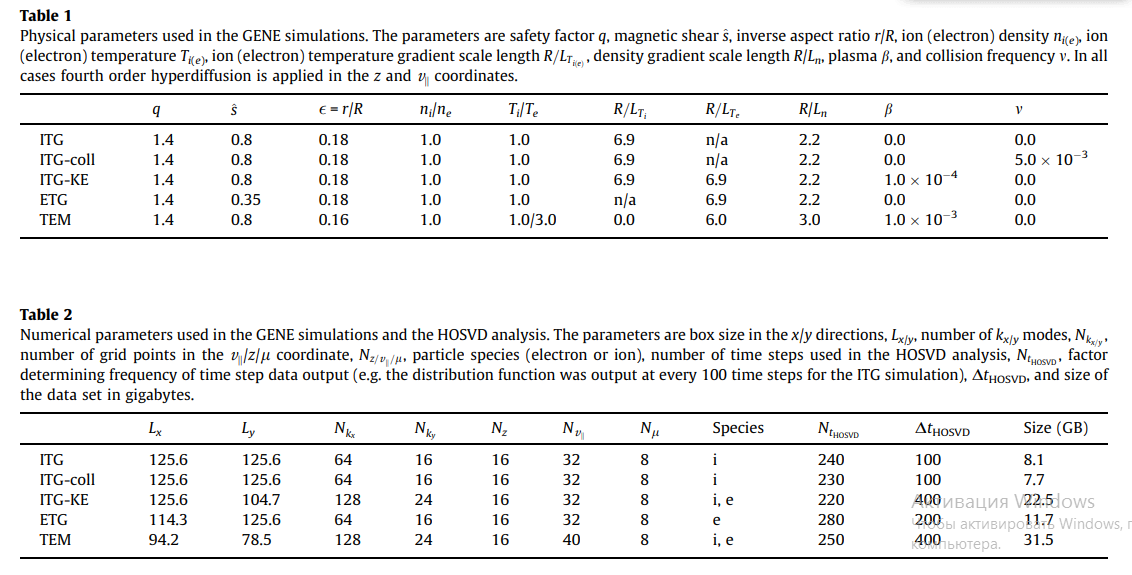
\includegraphics[width=1.2\textwidth]{sections/example/figures/gyrokinetic.png}
%\caption{Some description}
\label{fig:example:1}
\end{figure}

% сказать про многомерное преобразование фурье, известный метод, выбор моды, сравнение двух методов в снижении числа индексов тензора данных. 

\subsection{Experiment}
The implementation of HOSVD and the computational experiment from \cite{hatch2012analysis} can be found on GitHub repository\footnote{https://github.com/Tonchik-hv/Math-methods-of-forecasting}.

\subsection{Code analysis}

\begin{figure}[h]
\centering
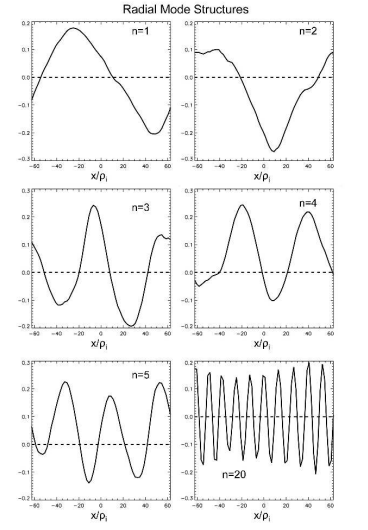
\includegraphics[width=1\textwidth]{sections/example/figures/mode_str.png}
\caption{Selected HOSVD mode structures for the radial (x) coordinate}
\label{fig:example:1}
\end{figure}

\begin{figure}[h]
\centering
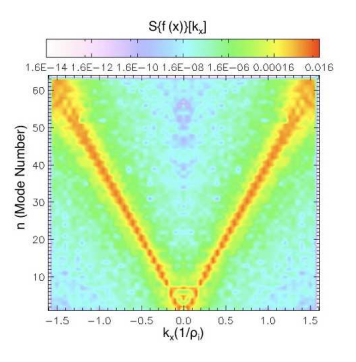
\includegraphics[width=1\textwidth]{sections/example/figures/plot.png}
\caption{Fourier spectra of the HOSVD x-modes. At low kx some modes represent multiple scales. At higher kx the modes largely correspond to single Fourier modes (note that δkxρs = 0.05).}
\label{fig:example:1}
\end{figure}


\begin{figure}[h]
\centering
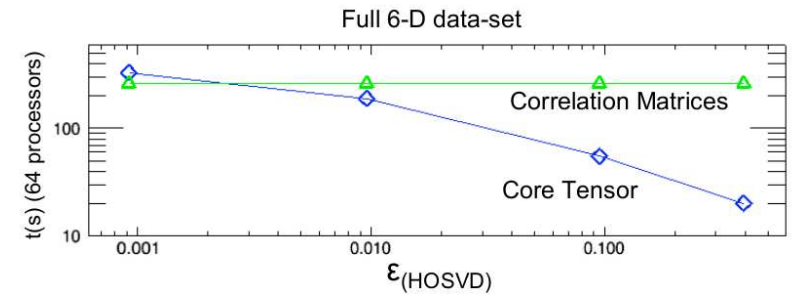
\includegraphics[width=1.2\textwidth]{sections/example/figures/error.png}
\caption{ Computation time to solve for the truncated core tensor against truncation error. Computation time for the construction of the correlation matrices.}
\label{fig:example:1}
\end{figure}




\end{document}
